% Options for packages loaded elsewhere
\PassOptionsToPackage{unicode}{hyperref}
\PassOptionsToPackage{hyphens}{url}
\documentclass[
  10pt,
  a4paper,
]{article}
\usepackage{xcolor}
\usepackage[margin=0.75in]{geometry}
\usepackage{amsmath,amssymb}
\setcounter{secnumdepth}{5}
\usepackage{iftex}
\ifPDFTeX
  \usepackage[T1]{fontenc}
  \usepackage[utf8]{inputenc}
  \usepackage{textcomp} % provide euro and other symbols
\else % if luatex or xetex
  \usepackage{unicode-math} % this also loads fontspec
  \defaultfontfeatures{Scale=MatchLowercase}
  \defaultfontfeatures[\rmfamily]{Ligatures=TeX,Scale=1}
\fi
\usepackage{lmodern}
\ifPDFTeX\else
  % xetex/luatex font selection
\fi
% Use upquote if available, for straight quotes in verbatim environments
\IfFileExists{upquote.sty}{\usepackage{upquote}}{}
\IfFileExists{microtype.sty}{% use microtype if available
  \usepackage[]{microtype}
  \UseMicrotypeSet[protrusion]{basicmath} % disable protrusion for tt fonts
}{}
\makeatletter
\@ifundefined{KOMAClassName}{% if non-KOMA class
  \IfFileExists{parskip.sty}{%
    \usepackage{parskip}
  }{% else
    \setlength{\parindent}{0pt}
    \setlength{\parskip}{6pt plus 2pt minus 1pt}}
}{% if KOMA class
  \KOMAoptions{parskip=half}}
\makeatother
\usepackage{longtable,booktabs,array}
\usepackage{calc} % for calculating minipage widths
% Correct order of tables after \paragraph or \subparagraph
\usepackage{etoolbox}
\makeatletter
\patchcmd\longtable{\par}{\if@noskipsec\mbox{}\fi\par}{}{}
\makeatother
% Allow footnotes in longtable head/foot
\IfFileExists{footnotehyper.sty}{\usepackage{footnotehyper}}{\usepackage{footnote}}
\makesavenoteenv{longtable}
\usepackage{graphicx}
\makeatletter
\newsavebox\pandoc@box
\newcommand*\pandocbounded[1]{% scales image to fit in text height/width
  \sbox\pandoc@box{#1}%
  \Gscale@div\@tempa{\textheight}{\dimexpr\ht\pandoc@box+\dp\pandoc@box\relax}%
  \Gscale@div\@tempb{\linewidth}{\wd\pandoc@box}%
  \ifdim\@tempb\p@<\@tempa\p@\let\@tempa\@tempb\fi% select the smaller of both
  \ifdim\@tempa\p@<\p@\scalebox{\@tempa}{\usebox\pandoc@box}%
  \else\usebox{\pandoc@box}%
  \fi%
}
% Set default figure placement to htbp
\def\fps@figure{htbp}
\makeatother
\setlength{\emergencystretch}{3em} % prevent overfull lines
\providecommand{\tightlist}{%
  \setlength{\itemsep}{0pt}\setlength{\parskip}{0pt}}
\usepackage[]{natbib}
\bibliographystyle{plainnat}
\usepackage{bookmark}
\IfFileExists{xurl.sty}{\usepackage{xurl}}{} % add URL line breaks if available
\urlstyle{same}
\hypersetup{
  pdftitle={Routing AI agents by software engineering role: an operational record of 5,871 runs},
  pdfauthor={Daniel Bo and the Reading Advantage engineering team},
  hidelinks,
  pdfcreator={LaTeX via pandoc}}

\title{Routing AI agents by software engineering role: an operational
record of 5,871 runs}
\author{Daniel Bo and the Reading Advantage engineering team}
\date{Reading Advantage (Thailand), Khon Kaen, Thailand}

\begin{document}
\maketitle

\textbf{Version:} v0.3\\
\textbf{Date:} 2026-11-27

\subsection*{Abstract}\label{abstract}
\addcontentsline{toc}{subsection}{Abstract}

Between June and November 2026, we examine 5,871 runs across 68 route
labels and 17 family labels in an engineering workflow. Records occur in
four months, with 87.2\% of runs in November; selection, repeated work
and missing verdicts limit comparisons. Producers passed 674 of 753
verdicts (89.5\%; Wilson 95\% interval 87.1 to 91.5\%; coverage 46.1\%).
Reviewers approved 2,681 of 3,516 verdicts (76.3\%; interval 74.8 to
77.6\%; coverage 82.9\%). We describe findings, rater scores, cost
classes and three routing trials: Jev instrumentation, Sonnet effort and
HungerG production. The benchmark supplement uses three HungerG runs per
arm; Arm A ranges overlap (92.8 to 95.7; historical DeepSeek 90.9 to
95.0). Arm B HungerG scores span 95.8 to 100.0; the historical reference
has a single score of 97.7. Different fixture revisions prevent
controlled comparisons across models; the operational record has no
routing baseline or evidence of routing benefit.

\section{Introduction}\label{introduction}

Agent-based software engineering changes the unit of model selection.
The orchestrator can assign a model to write tests and another to
implement the change. Other models check the change. Each assignment has
a different objective. A reviewer can reject an artifact and thereby
help the task succeed. An implementation agent must satisfy a contract
and produce working code.

A route is also a deployment choice. Providers can expose the same
family through different endpoints or effort settings. Route
availability and independent review constrain the choice. We study these
assignments in a spec-driven workflow called Measure. The records
include software engineering, documentation, curriculum work and
benchmark work.

We ask four questions of the records:

\begin{itemize}
\tightlist
\item
  \textbf{RQ1.} Do observed family-role differences persist when we
  examine missing verdicts and exclude individual directories?
\item
  \textbf{RQ2.} Do recorded finding frequencies differ when we restrict
  the denominator to decision runs?
\item
  \textbf{RQ3.} Do the observed route classes and months show a uniform
  distribution of recorded work?
\item
  \textbf{RQ4.} Do recorded rater scores and raw agreement provide
  independent evidence of artifact correctness?
\end{itemize}

\section{Setting}\label{setting}

\subsection{Spec-driven work and role
boundaries}\label{spec-driven-work-and-role-boundaries}

Measure divides work into tracks. Each track contains a specification
and a phased plan. The orchestrator assigns an agent a bounded task and
its evidence. A role specifies a responsibility. A route specifies an
endpoint and effort setting.

The strategy role prepares the implementation approach. The Red role
writes tests that should fail until the specified behavior exists. The
Green role implements the behavior and reruns the checks. The
orchestrator requests different families for Red and Green where the
independence rule applies. The coder, record and small roles perform
bounded tasks.

Review A checks correctness and architecture. Review B checks applicable
security and data risks. Review C checks interface and user flow
contracts. Adversarial testing checks edge cases and evidence. Spec
review checks the planned work. Vision review checks visual evidence.
Phase acceptance checks a phase at a fixed revision. Final acceptance
checks the completed track. We retain the separate acceptance label in
the records.

The role groups distinguish producers from decision roles. Decision
roles comprise review-a, review-b, review-c, adversarial, spec-review,
vision-review, acceptance, phase-acceptance and final-acceptance. All
other observed roles are producers. A producer pass records a work
result. A decision pass records an approval. Under the independence
rule, reviewers come from families other than the producer family. A
stricter reviewer can lower the recorded pass rate of the producers it
reviews. The export has no direct key that links a producer to reviewer
verdicts on its artifact. Shared sessions or task tags do not establish
that link.

A task can require implementation followed by review and correction. The
orchestrator can assign another run after a failed gate. A run is
therefore not a count of distinct tasks or defects.

\subsection{Route selection}\label{route-selection}

Project management is a role that sets or approves route policy. The
routing tool uses ordered route lists by role. It checks route
eligibility and availability. It also checks family exclusions for
independent review. The tool returns the first eligible route or reports
that none is available. Project management can record a substitution.

The policy changed during the period. On November 24, the
phase-acceptance effort policy moved away from max. We treat Sonnet
labels under \texttt{claude-code} and \texttt{claude-agent} as the same
recorded family. We do not assume that earlier assignments followed the
later policy.

\section{Data and method}\label{data-and-method}

\subsection{Population and
reproducibility}\label{population-and-reproducibility}

We select runs whose recorded start time is at or before
2026-11-26T22:21:52Z. The first record has start time
2026-06-06T23:43:33Z. The dataset contains 5,871 runs in 23 anonymous
directories and 15 roles. We retain all domains and legacy records.
Directory identifiers do not denote distinct projects.

The frozen SQLite copy, \texttt{outcomes-20261127T083716761728Z.sqlite},
dates to 2026-11-27T08:37Z. Its SHA-256 is:

\texttt{59eddd0eb34019870463451367f5f059a176331b00acab0beb30b295776e89b0}

The script \texttt{paper1\_tables.py} uses \texttt{-\/-from-snapshot}
and the cutoff to build the aggregates from the copy. Version v0.2 used
an earlier copy. The CSV arithmetic reproduces from the frozen copy. The
trial rows come from private files and contain counts and numeric
summaries only. The trial extract does not permit a recount of all
underlying private records.

We normalize a route by taking the first stored token and removing
trailing punctuation. The lookup then applies ordered string rules
without regard to case. Family denotes a label and can group multiple
routes. The label does not verify the executed model. Appendix A lists
the rules, examples and residual labels.

We classify domains by directory name. The map assigns code, markdown or
curriculum, and benchmark work. The classification of dir\_08 (302 runs)
and four additional directories with few runs is uncertain. The mixed
domain population limits the interpretation of pooled comparisons.

\subsection{Measures and analysis}\label{measures-and-analysis}

Let P be the number of passes, F the number of failures and N the number
of runs. A verdict is a pass or fail. The conditional rate is P/(P+F),
and coverage is (P+F)/N. We call the conditional rate an approval rate
for decision roles. The lower bound is P/N; the upper bound is (N−F)/N.
These bounds treat every run without a binary verdict as a failure or a
pass, respectively.

We group explicit no\_verdict and NULL results as no verdict. We group
error, timeout and abandoned results as errors. We retain all runs in N.
A conditional rate is undefined if no verdict exists.

We calculate percentages from integer counts and round once. We report
Wilson 95\% intervals for binary proportions. These intervals describe
run-level uncertainty and do not adjust for clustered observations. The
bounds describe missing outcomes and are not confidence intervals.
Repeated assignments and selective allocation prevent inference from an
independent random sample.

Table 1 includes every family-role cell with at least 30 verdicts.
Appendix B marks and reports cells below this minimum. The full 138-cell
table remains in \texttt{by\_family\_role.csv}. For each main cell, we
exclude each directory in turn and report the minimum and maximum
remaining rate. The sensitivity export stores these extrema to four
decimal places. This sensitivity analysis does not adjust for task
difficulty.

Finding frequencies use decision-role runs as the denominator. An escape
is a severity label: \texttt{escaped\ =\ 1} if and only if
\texttt{severity\ =\ escape}. We verified this relation for all 8,679
selected findings. Findings per run can exceed unity, so a binomial
Wilson interval does not apply to this frequency.

The rating rubric uses scores from 1 through 5. Model reviewers in
decision roles record scores; human judges do not supply these ratings.
The given view groups by rater route. The received view groups by the
family of the rated run. The data lack a direct link to the producer of
the rated artifact. Consequently, the received view cannot establish a
producer-family rating. Review accuracy and agreement describe the same
check. We report the agreement once, with the checker family.

The cost map records the route class at extraction. Subscription, credit
and free are classifications of routes. Unknown means the map lacks a
class. These classes do not measure spend or token consumption.

\section{Results}\label{results}

\subsection{RQ1: Family-role verdicts and
sensitivity}\label{rq1-family-role-verdicts-and-sensitivity}

The snapshot contains 3,355 passes and 914 failures. It contains 897
explicit no-verdict results and 622 NULL results. The error class
contains 70 errors, zero timeouts and 13 abandonments.

The aggregate role groups have the following outcomes. Coverage
intervals refer to all runs; conditional-rate intervals use verdicts.

\begin{longtable}[]{@{}
  >{\raggedright\arraybackslash}p{(\linewidth - 10\tabcolsep) * \real{0.1667}}
  >{\raggedleft\arraybackslash}p{(\linewidth - 10\tabcolsep) * \real{0.1667}}
  >{\raggedleft\arraybackslash}p{(\linewidth - 10\tabcolsep) * \real{0.1667}}
  >{\raggedleft\arraybackslash}p{(\linewidth - 10\tabcolsep) * \real{0.1667}}
  >{\raggedleft\arraybackslash}p{(\linewidth - 10\tabcolsep) * \real{0.1667}}
  >{\raggedleft\arraybackslash}p{(\linewidth - 10\tabcolsep) * \real{0.1667}}@{}}
\toprule\noalign{}
\begin{minipage}[b]{\linewidth}\raggedright
Role group
\end{minipage} & \begin{minipage}[b]{\linewidth}\raggedleft
P/V/N
\end{minipage} & \begin{minipage}[b]{\linewidth}\raggedleft
Coverage \% (CI)
\end{minipage} & \begin{minipage}[b]{\linewidth}\raggedleft
Rate \%
\end{minipage} & \begin{minipage}[b]{\linewidth}\raggedleft
CI \%
\end{minipage} & \begin{minipage}[b]{\linewidth}\raggedleft
Bounds \%
\end{minipage} \\
\midrule\noalign{}
\endhead
\bottomrule\noalign{}
\endlastfoot
producer & 674/753/1632 & 46.1 (43.7--48.6) & 89.5 & 87.1--91.5 &
41.3--95.2 \\
decision & 2681/3516/4239 & 82.9 (81.8--84.0) & 76.3 & 74.8--77.6 &
63.2--80.3 \\
\end{longtable}

Table 1 first lists producer cells and then decision cells. The coverage
of all Green runs is 46.6\% (319 of 685; CI 42.9--50.3\%). For all Red
runs, coverage is 48.8\% (202 of 414; CI 44.0--53.6\%). Producer
observations are partial. The table includes the missing-outcome bounds
and leave-one-directory-out range for each cell.

\begin{longtable}[]{@{}
  >{\raggedright\arraybackslash}p{(\linewidth - 14\tabcolsep) * \real{0.1250}}
  >{\raggedright\arraybackslash}p{(\linewidth - 14\tabcolsep) * \real{0.1250}}
  >{\raggedleft\arraybackslash}p{(\linewidth - 14\tabcolsep) * \real{0.1250}}
  >{\raggedleft\arraybackslash}p{(\linewidth - 14\tabcolsep) * \real{0.1250}}
  >{\raggedleft\arraybackslash}p{(\linewidth - 14\tabcolsep) * \real{0.1250}}
  >{\raggedleft\arraybackslash}p{(\linewidth - 14\tabcolsep) * \real{0.1250}}
  >{\raggedleft\arraybackslash}p{(\linewidth - 14\tabcolsep) * \real{0.1250}}
  >{\raggedleft\arraybackslash}p{(\linewidth - 14\tabcolsep) * \real{0.1250}}@{}}
\caption{Table 1. Family-role cells. P/V/N = passes/verdicts/runs. All
rate columns use percent. CI = Wilson interval; bounds = all missing
fail or pass; LOO = directory exclusion range.}\tabularnewline
\toprule\noalign{}
\begin{minipage}[b]{\linewidth}\raggedright
Role
\end{minipage} & \begin{minipage}[b]{\linewidth}\raggedright
Family
\end{minipage} & \begin{minipage}[b]{\linewidth}\raggedleft
P/V/N
\end{minipage} & \begin{minipage}[b]{\linewidth}\raggedleft
Cov.
\end{minipage} & \begin{minipage}[b]{\linewidth}\raggedleft
Rate
\end{minipage} & \begin{minipage}[b]{\linewidth}\raggedleft
CI
\end{minipage} & \begin{minipage}[b]{\linewidth}\raggedleft
Bounds
\end{minipage} & \begin{minipage}[b]{\linewidth}\raggedleft
LOO
\end{minipage} \\
\midrule\noalign{}
\endfirsthead
\toprule\noalign{}
\begin{minipage}[b]{\linewidth}\raggedright
Role
\end{minipage} & \begin{minipage}[b]{\linewidth}\raggedright
Family
\end{minipage} & \begin{minipage}[b]{\linewidth}\raggedleft
P/V/N
\end{minipage} & \begin{minipage}[b]{\linewidth}\raggedleft
Cov.
\end{minipage} & \begin{minipage}[b]{\linewidth}\raggedleft
Rate
\end{minipage} & \begin{minipage}[b]{\linewidth}\raggedleft
CI
\end{minipage} & \begin{minipage}[b]{\linewidth}\raggedleft
Bounds
\end{minipage} & \begin{minipage}[b]{\linewidth}\raggedleft
LOO
\end{minipage} \\
\midrule\noalign{}
\endhead
\bottomrule\noalign{}
\endlastfoot
green & deepseek & 101/111/239 & 46.4 & 91.0 & 84.2--95.0 & 42.3--95.8 &
88.9--92.2 \\
green & hy & 61/69/119 & 58.0 & 88.4 & 78.8--94.0 & 51.3--93.3 &
87.3--90.4 \\
green & minimax & 63/71/150 & 47.3 & 88.7 & 79.3--94.2 & 42.0--94.7 &
86.9--90.6 \\
green & muse & 23/45/99 & 45.5 & 51.1 & 37.0--65.0 & 23.2--77.8 &
40.5--91.3 \\
record & hy & 29/31/51 & 60.8 & 93.5 & 79.3--98.2 & 56.9--96.1 &
90.9--96.3 \\
record & minimax & 29/32/56 & 57.1 & 90.6 & 75.8--96.8 & 51.8--94.6 &
85.7--93.3 \\
red & deepseek & 29/31/71 & 43.7 & 93.5 & 79.3--98.2 & 40.8--97.2 &
92.6--96.2 \\
red & muse & 120/129/196 & 65.8 & 93.0 & 87.3--96.3 & 61.2--95.4 &
92.2--94.8 \\
strategy & hy & 33/34/49 & 69.4 & 97.1 & 85.1--99.5 & 67.3--98.0 &
96.2--100.0 \\
adversarial & claude & 26/42/50 & 84.0 & 61.9 & 46.8--75.0 & 52.0--68.0
& 60.0--66.7 \\
adversarial & glm & 34/52/60 & 86.7 & 65.4 & 51.8--76.8 & 56.7--70.0 &
60.0--78.4 \\
adversarial & hy & 22/35/46 & 76.1 & 62.9 & 46.3--76.8 & 47.8--71.7 &
58.1--81.2 \\
adversarial & muse & 20/37/41 & 90.2 & 54.1 & 38.4--69.0 & 48.8--58.5 &
50.0--58.6 \\
adversarial & openai & 64/99/109 & 90.8 & 64.6 & 54.8--73.4 & 58.7--67.9
& 60.0--71.1 \\
adversarial & unknown & 133/158/164 & 96.3 & 84.2 & 77.7--89.0 &
81.1--84.8 & 78.0--87.0 \\
phase-acceptance & claude & 120/146/165 & 88.5 & 82.2 & 75.2--87.5 &
72.7--84.2 & 79.4--84.1 \\
phase-acceptance & glm & 42/45/56 & 80.4 & 93.3 & 82.1--97.7 &
75.0--94.6 & 90.6--97.4 \\
phase-acceptance & openai & 34/59/64 & 92.2 & 57.6 & 44.9--69.4 &
53.1--60.9 & 51.1--63.3 \\
phase-acceptance & unknown & 143/153/156 & 98.1 & 93.5 & 88.4--96.4 &
91.7--93.6 & 91.2--96.4 \\
review-a & claude & 96/133/149 & 89.3 & 72.2 & 64.0--79.1 & 64.4--75.2 &
70.6--74.7 \\
review-a & deepseek & 54/71/120 & 59.2 & 76.1 & 65.0--84.5 & 45.0--85.8
& 70.0--88.5 \\
review-a & glm & 75/97/120 & 80.8 & 77.3 & 68.0--84.5 & 62.5--81.7 &
73.2--85.0 \\
review-a & mimo & 59/73/85 & 85.9 & 80.8 & 70.3--88.2 & 69.4--83.5 &
78.0--83.9 \\
review-a & minimax & 60/89/105 & 84.8 & 67.4 & 57.1--76.3 & 57.1--72.4 &
62.3--70.6 \\
review-a & muse & 47/53/76 & 69.7 & 88.7 & 77.4--94.7 & 61.8--92.1 &
87.2--91.3 \\
review-a & openai & 197/358/408 & 87.7 & 55.0 & 49.8--60.1 & 48.3--60.5
& 53.7--58.4 \\
review-a & unknown & 250/310/322 & 96.3 & 80.6 & 75.9--84.7 & 77.6--81.4
& 79.8--81.4 \\
review-b & claude & 45/53/67 & 79.1 & 84.9 & 72.9--92.1 & 67.2--88.1 &
82.6--86.7 \\
review-b & deepseek & 34/46/68 & 67.6 & 73.9 & 59.7--84.4 & 50.0--82.4 &
68.8--85.0 \\
review-b & glm & 33/37/47 & 78.7 & 89.2 & 75.3--95.7 & 70.2--91.5 &
88.0--92.0 \\
review-b & hy & 39/45/86 & 52.3 & 86.7 & 73.8--93.7 & 45.3--93.0 &
82.9--97.1 \\
review-b & kimi & 93/109/122 & 89.3 & 85.3 & 77.5--90.8 & 76.2--86.9 &
81.6--87.9 \\
review-b & unknown & 142/179/182 & 98.4 & 79.3 & 72.8--84.6 & 78.0--79.7
& 75.4--82.0 \\
review-c & claude & 43/56/60 & 93.3 & 76.8 & 64.2--85.9 & 71.7--78.3 &
74.5--80.0 \\
review-c & glm & 40/54/72 & 75.0 & 74.1 & 61.1--83.9 & 55.6--80.6 &
68.9--78.6 \\
review-c & muse & 29/30/42 & 71.4 & 96.7 & 83.3--99.4 & 69.0--97.6 &
92.9--100.0 \\
review-c & openai & 84/114/138 & 82.6 & 73.7 & 64.9--80.9 & 60.9--78.3 &
69.7--80.6 \\
review-c & unknown & 170/194/197 & 98.5 & 87.6 & 82.3--91.5 & 86.3--87.8
& 85.4--90.2 \\
\end{longtable}

The worked example shows the concentration of verdicts in dir\_03. Muse
Green passed 23 of 45 verdicts overall. Within dir\_03 it passed 2 of 22
verdicts; outside it passed 21 of 23 (91.3\%). The failures within that
directory occurred from November 20 to 22. The two busiest dates account
for 19 of the cell's 22 failures.

The free DeepSeek route shows the same concentration. It passed 2 of 33
verdicts inside dir\_03 and 31 of 45 (68.9\%) outside. The same
directory contributes failures to both cells. The directory split in
Table 2 shows why the overall cell rates cannot establish stable role or
route effects.

\begin{longtable}[]{@{}llrrrr@{}}
\caption{Table 2. Directory sensitivity example. An asterisk marks fewer
than 30 verdicts. Rates, coverage and intervals use
percent.}\tabularnewline
\toprule\noalign{}
Cell & Scope & P/V/N & Cov. & Rate & CI \\
\midrule\noalign{}
\endfirsthead
\toprule\noalign{}
Cell & Scope & P/V/N & Cov. & Rate & CI \\
\midrule\noalign{}
\endhead
\bottomrule\noalign{}
\endlastfoot
Muse Green & inside * & 2/22/26 & 84.6 & 9.1 & 2.5--27.8 \\
Muse Green & outside * & 21/23/73 & 31.5 & 91.3 & 73.2--97.6 \\
DeepSeek free & inside & 2/33/35 & 94.3 & 6.1 & 1.7--19.6 \\
DeepSeek free & outside & 31/45/149 & 30.2 & 68.9 & 54.3--80.5 \\
\end{longtable}

Figure 1 displays selected producer verdicts and their run-level
intervals before directory exclusion. The figure alone cannot show the
cluster effects that Table 2 describes.

\begin{figure}
\centering
\pandocbounded{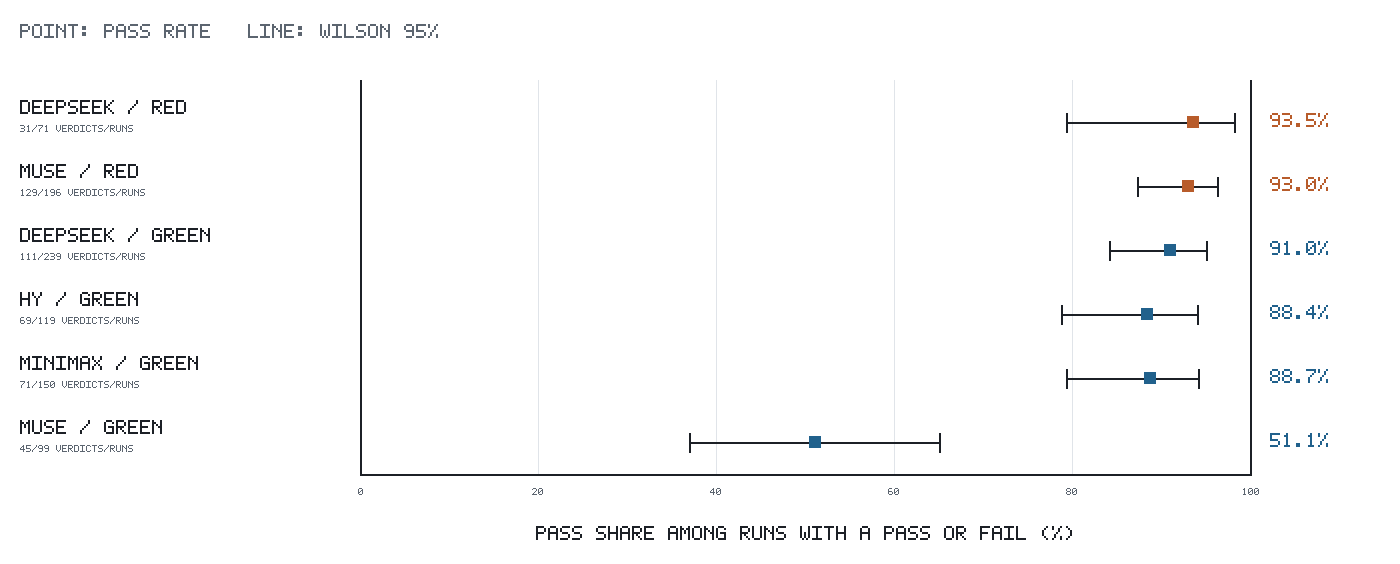
\includegraphics[keepaspectratio,alt={Figure 1. Selected producer verdicts and run-level Wilson intervals. The denominator below each label gives verdicts over runs.}]{figures/role-pass.png}}
\caption{Figure 1. Selected producer verdicts and run-level Wilson
intervals. The denominator below each label gives verdicts over runs.}
\end{figure}

Decision roles have a different objective. A lower approval rate can
indicate more stringent checks or more difficult work. It can also
indicate poor review performance. The records cannot distinguish these
explanations.

Table 3 separates the domain and role groups. The producer and decision
rates differ in each domain. These differences are descriptive because
the tasks differ.

\begin{longtable}[]{@{}
  >{\raggedright\arraybackslash}p{(\linewidth - 12\tabcolsep) * \real{0.1429}}
  >{\raggedright\arraybackslash}p{(\linewidth - 12\tabcolsep) * \real{0.1429}}
  >{\raggedleft\arraybackslash}p{(\linewidth - 12\tabcolsep) * \real{0.1429}}
  >{\raggedleft\arraybackslash}p{(\linewidth - 12\tabcolsep) * \real{0.1429}}
  >{\raggedleft\arraybackslash}p{(\linewidth - 12\tabcolsep) * \real{0.1429}}
  >{\raggedleft\arraybackslash}p{(\linewidth - 12\tabcolsep) * \real{0.1429}}
  >{\raggedleft\arraybackslash}p{(\linewidth - 12\tabcolsep) * \real{0.1429}}@{}}
\caption{Table 3. Domain and role group. Share is the share of all runs.
Coverage and conditional rates use percent.}\tabularnewline
\toprule\noalign{}
\begin{minipage}[b]{\linewidth}\raggedright
Domain
\end{minipage} & \begin{minipage}[b]{\linewidth}\raggedright
Group
\end{minipage} & \begin{minipage}[b]{\linewidth}\raggedleft
P/V/N
\end{minipage} & \begin{minipage}[b]{\linewidth}\raggedleft
Cov.
\end{minipage} & \begin{minipage}[b]{\linewidth}\raggedleft
Rate
\end{minipage} & \begin{minipage}[b]{\linewidth}\raggedleft
CI
\end{minipage} & \begin{minipage}[b]{\linewidth}\raggedleft
Share
\end{minipage} \\
\midrule\noalign{}
\endfirsthead
\toprule\noalign{}
\begin{minipage}[b]{\linewidth}\raggedright
Domain
\end{minipage} & \begin{minipage}[b]{\linewidth}\raggedright
Group
\end{minipage} & \begin{minipage}[b]{\linewidth}\raggedleft
P/V/N
\end{minipage} & \begin{minipage}[b]{\linewidth}\raggedleft
Cov.
\end{minipage} & \begin{minipage}[b]{\linewidth}\raggedleft
Rate
\end{minipage} & \begin{minipage}[b]{\linewidth}\raggedleft
CI
\end{minipage} & \begin{minipage}[b]{\linewidth}\raggedleft
Share
\end{minipage} \\
\midrule\noalign{}
\endhead
\bottomrule\noalign{}
\endlastfoot
benchmark & decision & 277/371/449 & 82.6 & 74.7 & 70.0--78.8 & 7.6 \\
benchmark & producer & 69/75/175 & 42.9 & 92.0 & 83.6--96.3 & 3.0 \\
code & decision & 1582/2104/2443 & 86.1 & 75.2 & 73.3--77.0 & 41.6 \\
code & producer & 379/439/840 & 52.3 & 86.3 & 82.8--89.2 & 14.3 \\
markdown/curriculum & decision & 822/1041/1347 & 77.3 & 79.0 &
76.4--81.3 & 22.9 \\
markdown/curriculum & producer & 226/239/617 & 38.7 & 94.6 & 90.9--96.8
& 10.5 \\
\end{longtable}

\subsection{RQ2: Recorded findings}\label{rq2-recorded-findings}

Table 4 uses the decision-run denominator for each family. It includes
findings that the decision run records, rather than a count of distinct
defects. The observed frequencies differ even with that denominator.
Escape frequencies do not identify which family missed a defect at an
earlier gate.

\begin{longtable}[]{@{}lrrrrrr@{}}
\caption{Table 4. Findings and escapes per decision run. Coverage refers
to verdicts on decision runs. Findings and escapes are event counts, not
binary proportions. An asterisk marks fewer than 30
verdicts.}\tabularnewline
\toprule\noalign{}
Family & Runs & Cov. \% & Findings & Escapes & F/run & E/100 \\
\midrule\noalign{}
\endfirsthead
\toprule\noalign{}
Family & Runs & Cov. \% & Findings & Escapes & F/run & E/100 \\
\midrule\noalign{}
\endhead
\bottomrule\noalign{}
\endlastfoot
beam * & 30 & 80.0 & 19 & 6 & 0.63 & 20.0 \\
claude & 553 & 85.2 & 1848 & 10 & 3.34 & 1.8 \\
deepseek & 348 & 55.7 & 347 & 15 & 1.00 & 4.3 \\
doubao * & 1 & 100.0 & 2 & 0 & 2.00 & 0.0 \\
glm & 373 & 77.5 & 556 & 12 & 1.49 & 3.2 \\
hy & 155 & 61.3 & 42 & 15 & 0.27 & 9.7 \\
kimi & 224 & 85.3 & 263 & 15 & 1.17 & 6.7 \\
mimo & 153 & 77.1 & 287 & 7 & 1.88 & 4.6 \\
minimax & 206 & 80.1 & 437 & 18 & 2.12 & 8.7 \\
muse & 235 & 76.6 & 292 & 5 & 1.24 & 2.1 \\
nemotron * & 1 & 0.0 & 0 & 0 & 0.00 & 0.0 \\
openai & 796 & 84.4 & 1061 & 61 & 1.33 & 7.7 \\
other-cn-infra * & 2 & 100.0 & 3 & 1 & 1.50 & 50.0 \\
qwen & 37 & 81.1 & 97 & 5 & 2.62 & 13.5 \\
stepfun & 78 & 83.3 & 126 & 5 & 1.62 & 6.4 \\
unknown & 1047 & 97.3 & 3299 & 50 & 3.15 & 4.8 \\
\end{longtable}

Different opportunities to inspect artifacts can change the frequencies.
The unknown family also contains legacy severity labels that differ from
the current taxonomy. We have no common set of defects against which to
estimate precision or recall.

\subsection{RQ3: Cost classes and record
periods}\label{rq3-cost-classes-and-record-periods}

Table 5 reports the observed distribution under the extraction-time
route map. The unknown class covers 1,291 runs on 20 routes. It includes
1,047 legacy unknown-family runs and 244 runs on 19 named routes without
a mapping. One Muse route accounts for 609 of the 616 credit-class runs.
Class shares do not quantify cost differences. We do not compare
conditional pass rates by cost class.

\begin{longtable}[]{@{}lrrrrr@{}}
\caption{Table 5. Route classes. Share and verdict coverage use percent.
Intervals refer to the share of runs in each class.}\tabularnewline
\toprule\noalign{}
Class & Runs & Routes & Share & Share CI & Cov. \\
\midrule\noalign{}
\endfirsthead
\toprule\noalign{}
Class & Runs & Routes & Share & Share CI & Cov. \\
\midrule\noalign{}
\endhead
\bottomrule\noalign{}
\endlastfoot
credit & 616 & 3 & 10.5 & 9.7--11.3 & 62.0 \\
free & 828 & 13 & 14.1 & 13.2--15.0 & 55.9 \\
subscription & 3136 & 32 & 53.4 & 52.1--54.7 & 72.4 \\
unknown & 1291 & 20 & 22.0 & 20.9--23.1 & 89.2 \\
\end{longtable}

Figure 2 shows records in June, August, October and November. It
includes the months with no records and marks November as partial.
November accounts for 5,118 of 5,871 records (87.2\%). June and August
records carry the unknown family label; the composition of subsequent
records differs.

\begin{figure}
\centering
\pandocbounded{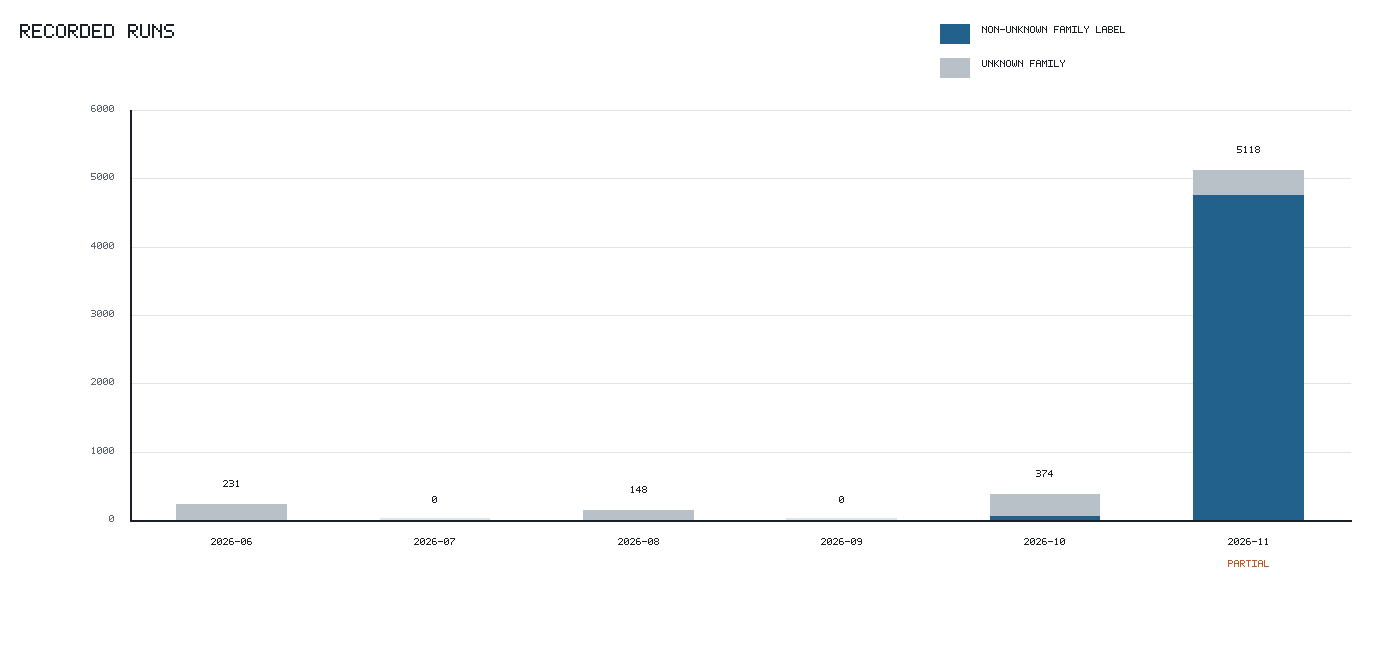
\includegraphics[keepaspectratio,alt={Figure 2. Monthly record volume, including zero-record months. November is partial.}]{figures/monthly-runs.png}}
\caption{Figure 2. Monthly record volume, including zero-record months.
November is partial.}
\end{figure}

Table 6 gives the period counts and the pooled sensitivity comparison.
The unknown label accounts for 1,047 runs and has no explicit no-verdict
or NULL results. It still contains errors. The non-unknown population
excludes these legacy rows, but retains residual labels. The pooled rate
combines unlike outcomes and primarily describes the November policy.

\begin{longtable}[]{@{}
  >{\raggedright\arraybackslash}p{(\linewidth - 10\tabcolsep) * \real{0.1667}}
  >{\raggedleft\arraybackslash}p{(\linewidth - 10\tabcolsep) * \real{0.1667}}
  >{\raggedleft\arraybackslash}p{(\linewidth - 10\tabcolsep) * \real{0.1667}}
  >{\raggedleft\arraybackslash}p{(\linewidth - 10\tabcolsep) * \real{0.1667}}
  >{\raggedleft\arraybackslash}p{(\linewidth - 10\tabcolsep) * \real{0.1667}}
  >{\raggedleft\arraybackslash}p{(\linewidth - 10\tabcolsep) * \real{0.1667}}@{}}
\caption{Table 6. Months and population sensitivity. P/V/N =
passes/verdicts/runs. The pooled rates combine producer passes and
decision approvals.}\tabularnewline
\toprule\noalign{}
\begin{minipage}[b]{\linewidth}\raggedright
Population
\end{minipage} & \begin{minipage}[b]{\linewidth}\raggedleft
P/V/N
\end{minipage} & \begin{minipage}[b]{\linewidth}\raggedleft
Cov. \%
\end{minipage} & \begin{minipage}[b]{\linewidth}\raggedleft
Rate \%
\end{minipage} & \begin{minipage}[b]{\linewidth}\raggedleft
CI \%
\end{minipage} & \begin{minipage}[b]{\linewidth}\raggedleft
Bounds \%
\end{minipage} \\
\midrule\noalign{}
\endfirsthead
\toprule\noalign{}
\begin{minipage}[b]{\linewidth}\raggedright
Population
\end{minipage} & \begin{minipage}[b]{\linewidth}\raggedleft
P/V/N
\end{minipage} & \begin{minipage}[b]{\linewidth}\raggedleft
Cov. \%
\end{minipage} & \begin{minipage}[b]{\linewidth}\raggedleft
Rate \%
\end{minipage} & \begin{minipage}[b]{\linewidth}\raggedleft
CI \%
\end{minipage} & \begin{minipage}[b]{\linewidth}\raggedleft
Bounds \%
\end{minipage} \\
\midrule\noalign{}
\endhead
\bottomrule\noalign{}
\endlastfoot
2026-06 & 222/230/231 & 99.6 & 96.5 & 93.3--98.2 & 96.1--96.5 \\
2026-07 & 0/0/0 & --- & --- & --- & --- \\
2026-08 & 146/148/148 & 100.0 & 98.6 & 95.2--99.6 & 98.6--98.6 \\
2026-09 & 0/0/0 & --- & --- & --- & --- \\
2026-10 & 266/361/374 & 96.5 & 73.7 & 68.9--78.0 & 71.1--74.6 \\
2026-11 & 2721/3530/5118 & 69.0 & 77.1 & 75.7--78.4 & 53.2--84.2 \\
Pooled & 3355/4269/5871 & 72.7 & 78.6 & 77.3--79.8 & 57.1--84.4 \\
Without unknown & 2496/3250/4824 & 67.4 & 76.8 & 75.3--78.2 &
51.7--84.4 \\
Unknown only & 859/1019/1047 & 97.3 & 84.3 & 81.9--86.4 & 82.0--84.7 \\
\end{longtable}

\subsection{RQ4: Recorded rater scores}\label{rq4-recorded-rater-scores}

Tables 7 and 8 report the axes for correctness, evidence quality, scope
discipline and test meaning. They give medians and the share of scores
at or below 3. The two Muse evidence labels have different names. We
retain them separately. The exporter renamed four Muse test\_mean rows
to test\_meaning and kept their evidence unchanged. Consequently, Muse
has different counts by axis.

\begin{longtable}[]{@{}
  >{\raggedright\arraybackslash}p{(\linewidth - 8\tabcolsep) * \real{0.2000}}
  >{\raggedleft\arraybackslash}p{(\linewidth - 8\tabcolsep) * \real{0.2000}}
  >{\raggedleft\arraybackslash}p{(\linewidth - 8\tabcolsep) * \real{0.2000}}
  >{\raggedleft\arraybackslash}p{(\linewidth - 8\tabcolsep) * \real{0.2000}}
  >{\raggedleft\arraybackslash}p{(\linewidth - 8\tabcolsep) * \real{0.2000}}@{}}
\caption{Table 7. Scores given by rater family. Each cell reports n;
median; percent at or below 3 (Wilson interval). An asterisk marks n
below 30.}\tabularnewline
\toprule\noalign{}
\begin{minipage}[b]{\linewidth}\raggedright
Family
\end{minipage} & \begin{minipage}[b]{\linewidth}\raggedleft
Correctness
\end{minipage} & \begin{minipage}[b]{\linewidth}\raggedleft
Evidence quality
\end{minipage} & \begin{minipage}[b]{\linewidth}\raggedleft
Scope discipline
\end{minipage} & \begin{minipage}[b]{\linewidth}\raggedleft
Test meaning
\end{minipage} \\
\midrule\noalign{}
\endfirsthead
\toprule\noalign{}
\begin{minipage}[b]{\linewidth}\raggedright
Family
\end{minipage} & \begin{minipage}[b]{\linewidth}\raggedleft
Correctness
\end{minipage} & \begin{minipage}[b]{\linewidth}\raggedleft
Evidence quality
\end{minipage} & \begin{minipage}[b]{\linewidth}\raggedleft
Scope discipline
\end{minipage} & \begin{minipage}[b]{\linewidth}\raggedleft
Test meaning
\end{minipage} \\
\midrule\noalign{}
\endhead
\bottomrule\noalign{}
\endlastfoot
beam & 8*; 5; 0.0 (0.0--32.4) & 8*; 5; 0.0 (0.0--32.4) & 8*; 5; 0.0
(0.0--32.4) & 8*; 5; 12.5 (2.2--47.1) \\
claude & 239; 4; 20.5 (15.9--26.1) & 239; 4; 8.8 (5.8--13.1) & 239; 5;
0.8 (0.2--3.0) & 239; 4; 33.9 (28.2--40.1) \\
deepseek & 46; 4; 21.7 (12.3--35.6) & 46; 5; 8.7 (3.4--20.3) & 46; 5;
0.0 (0.0--7.7) & 46; 4; 28.3 (17.3--42.5) \\
glm & 172; 5; 10.5 (6.7--15.9) & 172; 5; 2.9 (1.2--6.6) & 172; 5; 0.0
(0.0--2.2) & 172; 4; 14.0 (9.6--19.9) \\
hy & 24*; 5; 8.3 (2.3--25.8) & 24*; 5; 0.0 (0.0--13.8) & 24*; 5; 0.0
(0.0--13.8) & 24*; 4; 4.2 (0.7--20.2) \\
kimi & 108; 5; 20.4 (13.9--28.9) & 108; 5; 1.9 (0.5--6.5) & 108; 5; 0.0
(0.0--3.4) & 108; 4; 14.8 (9.3--22.7) \\
mimo & 68; 4; 16.2 (9.3--26.7) & 68; 5; 1.5 (0.3--7.9) & 68; 5; 0.0
(0.0--5.3) & 68; 4; 20.6 (12.7--31.6) \\
minimax & 67; 4; 26.9 (17.7--38.5) & 67; 4; 3.0 (0.8--10.2) & 67; 5; 0.0
(0.0--5.4) & 67; 4; 22.4 (14.1--33.7) \\
muse & 104; 5; 11.5 (6.7--19.1) & 102; 5; 0.0 (0.0--3.6) & 104; 5; 1.0
(0.2--5.2) & 104; 5; 2.9 (1.0--8.1) \\
openai & 442; 4; 38.7 (34.3--43.3) & 442; 5; 7.9 (5.7--10.8) & 442; 5;
2.7 (1.6--4.7) & 442; 4; 35.3 (31.0--39.9) \\
other-cn-infra & 2*; 4; 50.0 (9.5--90.5) & 2*; 5; 0.0 (0.0--65.8) & 2*;
5; 0.0 (0.0--65.8) & 2*; 4; 0.0 (0.0--65.8) \\
qwen & 18*; 5; 0.0 (0.0--17.6) & 18*; 5; 0.0 (0.0--17.6) & 18*; 5; 0.0
(0.0--17.6) & 18*; 4; 0.0 (0.0--17.6) \\
stepfun & 24*; 5; 16.7 (6.7--35.9) & 24*; 5; 4.2 (0.7--20.2) & 24*; 5;
0.0 (0.0--13.8) & 24*; 5; 12.5 (4.3--31.0) \\
unknown & 66; 4; 36.4 (25.8--48.4) & 66; 4.5; 4.5 (1.6--12.5) & 66; 5;
1.5 (0.3--8.1) & 66; 4; 31.8 (21.8--43.8) \\
muse: evidence & --- & 2*; 4; 0.0 (0.0--65.8) & --- & --- \\
\end{longtable}

\begin{longtable}[]{@{}
  >{\raggedright\arraybackslash}p{(\linewidth - 8\tabcolsep) * \real{0.2000}}
  >{\raggedleft\arraybackslash}p{(\linewidth - 8\tabcolsep) * \real{0.2000}}
  >{\raggedleft\arraybackslash}p{(\linewidth - 8\tabcolsep) * \real{0.2000}}
  >{\raggedleft\arraybackslash}p{(\linewidth - 8\tabcolsep) * \real{0.2000}}
  >{\raggedleft\arraybackslash}p{(\linewidth - 8\tabcolsep) * \real{0.2000}}@{}}
\caption{Table 8. Scores received by the family of the rated run. Each
cell reports n; median; percent at or below 3 (Wilson interval). These
are not producer-family scores.}\tabularnewline
\toprule\noalign{}
\begin{minipage}[b]{\linewidth}\raggedright
Family
\end{minipage} & \begin{minipage}[b]{\linewidth}\raggedleft
Correctness
\end{minipage} & \begin{minipage}[b]{\linewidth}\raggedleft
Evidence quality
\end{minipage} & \begin{minipage}[b]{\linewidth}\raggedleft
Scope discipline
\end{minipage} & \begin{minipage}[b]{\linewidth}\raggedleft
Test meaning
\end{minipage} \\
\midrule\noalign{}
\endfirsthead
\toprule\noalign{}
\begin{minipage}[b]{\linewidth}\raggedright
Family
\end{minipage} & \begin{minipage}[b]{\linewidth}\raggedleft
Correctness
\end{minipage} & \begin{minipage}[b]{\linewidth}\raggedleft
Evidence quality
\end{minipage} & \begin{minipage}[b]{\linewidth}\raggedleft
Scope discipline
\end{minipage} & \begin{minipage}[b]{\linewidth}\raggedleft
Test meaning
\end{minipage} \\
\midrule\noalign{}
\endhead
\bottomrule\noalign{}
\endlastfoot
beam & 8*; 5; 0.0 (0.0--32.4) & 8*; 5; 0.0 (0.0--32.4) & 8*; 5; 0.0
(0.0--32.4) & 8*; 5; 12.5 (2.2--47.1) \\
claude & 245; 4; 20.0 (15.5--25.5) & 245; 4; 8.6 (5.7--12.7) & 245; 5;
0.8 (0.2--2.9) & 245; 4; 33.5 (27.9--39.6) \\
deepseek & 46; 4; 21.7 (12.3--35.6) & 46; 5; 8.7 (3.4--20.3) & 46; 5;
0.0 (0.0--7.7) & 46; 4; 28.3 (17.3--42.5) \\
glm & 172; 5; 10.5 (6.7--15.9) & 172; 5; 2.9 (1.2--6.6) & 172; 5; 0.0
(0.0--2.2) & 172; 4; 14.0 (9.6--19.9) \\
hy & 24*; 5; 8.3 (2.3--25.8) & 24*; 5; 0.0 (0.0--13.8) & 24*; 5; 0.0
(0.0--13.8) & 24*; 4; 4.2 (0.7--20.2) \\
kimi & 108; 5; 20.4 (13.9--28.9) & 108; 5; 1.9 (0.5--6.5) & 108; 5; 0.0
(0.0--3.4) & 108; 4; 14.8 (9.3--22.7) \\
mimo & 68; 4; 16.2 (9.3--26.7) & 68; 5; 1.5 (0.3--7.9) & 68; 5; 0.0
(0.0--5.3) & 68; 4; 20.6 (12.7--31.6) \\
minimax & 67; 4; 26.9 (17.7--38.5) & 67; 4; 3.0 (0.8--10.2) & 67; 5; 0.0
(0.0--5.4) & 67; 4; 22.4 (14.1--33.7) \\
muse & 104; 5; 11.5 (6.7--19.1) & 102; 5; 0.0 (0.0--3.6) & 104; 5; 1.0
(0.2--5.2) & 104; 5; 2.9 (1.0--8.1) \\
openai & 442; 4; 38.7 (34.3--43.3) & 442; 5; 7.9 (5.7--10.8) & 442; 5;
2.7 (1.6--4.7) & 442; 4; 35.3 (31.0--39.9) \\
other-cn-infra & 2*; 4; 50.0 (9.5--90.5) & 2*; 5; 0.0 (0.0--65.8) & 2*;
5; 0.0 (0.0--65.8) & 2*; 4; 0.0 (0.0--65.8) \\
qwen & 18*; 5; 0.0 (0.0--17.6) & 18*; 5; 0.0 (0.0--17.6) & 18*; 5; 0.0
(0.0--17.6) & 18*; 4; 0.0 (0.0--17.6) \\
stepfun & 24*; 5; 16.7 (6.7--35.9) & 24*; 5; 4.2 (0.7--20.2) & 24*; 5;
0.0 (0.0--13.8) & 24*; 5; 12.5 (4.3--31.0) \\
unknown & 60; 4; 40.0 (28.6--52.6) & 60; 5; 5.0 (1.7--13.7) & 60; 5; 1.7
(0.3--8.9) & 60; 4; 33.3 (22.7--45.9) \\
muse: evidence & --- & 2*; 4; 0.0 (0.0--65.8) & --- & --- \\
\end{longtable}

The agreement checks are a separate interpretation of the
review-accuracy measure. They do not supply independent observations.
Table 9 groups them by checker family and includes the median
review-accuracy score given by that checker family. We can also group
checks by the family of the reviewer run. In this grouping, checks of
Muse reviews show agreement on 25 of 31 checks (80.6\%; CI
63.7--90.8\%). The checker-family grouping gives a different Muse count.
Agreement cannot establish correctness because both models can agree on
an incorrect judgment.

\begin{longtable}[]{@{}lrrrrrr@{}}
\caption{Table 9. Review agreement by checker family. Score columns
describe review-accuracy scores given by the checker. Agreement uses
agreed plus disagreed checks. An asterisk marks fewer than 30
checks.}\tabularnewline
\toprule\noalign{}
Checker & Agreed & Disagreed & Agree \% & CI \% & Median & ≤3 \% (CI) \\
\midrule\noalign{}
\endfirsthead
\toprule\noalign{}
Checker & Agreed & Disagreed & Agree \% & CI \% & Median & ≤3 \% (CI) \\
\midrule\noalign{}
\endhead
\bottomrule\noalign{}
\endlastfoot
claude & 193 & 13 & 93.7 & 89.5--96.3 & 4 & 10.7 (7.2--15.6) \\
deepseek * & 3 & 0 & 100.0 & 43.9--100.0 & 5 & 0.0 (0.0--56.1) \\
glm & 90 & 0 & 100.0 & 95.9--100.0 & 5 & 0.0 (0.0--4.1) \\
kimi * & 9 & 2 & 81.8 & 52.3--94.9 & 4 & 36.4 (15.2--64.6) \\
mimo * & 4 & 0 & 100.0 & 51.0--100.0 & 4.5 & 0.0 (0.0--49.0) \\
minimax * & 10 & 0 & 100.0 & 72.2--100.0 & 4 & 0.0 (0.0--27.8) \\
muse & 38 & 1 & 97.4 & 86.8--99.5 & 5 & 2.6 (0.5--13.2) \\
openai & 94 & 27 & 77.7 & 69.5--84.2 & 4 & 29.8 (22.3--38.4) \\
qwen * & 6 & 2 & 75.0 & 40.9--92.9 & 5 & 25.0 (7.1--59.1) \\
stepfun * & 19 & 0 & 100.0 & 83.2--100.0 & 5 & 0.0 (0.0--16.8) \\
unknown * & 19 & 1 & 95.0 & 76.4--99.1 & 5 & 5.0 (0.9--23.6) \\
\end{longtable}

\section{Three routing trials}\label{three-routing-trials}

\subsection{Jev shadow routing: instrumentation
result}\label{jev-shadow-routing-instrumentation-result}

Jev is a decision model that selects an eligible route from a task
description and route menu. The original script retained control of live
assignments during the shadow trial. The trial began on November 2 with
a planned duration of four days. The hook skipped the call when task
text was absent.

The initial period contained 398 decisions, including 211 without task
text (53.0\%; CI 48.1--57.9\%). Table 10 accounts for the cumulative
report after the atomic-mode extension. The original period and
cumulative period have different denominators. The cumulative share
without task text is 85.7\% (1,488 of 1,736; CI 84.0--87.3\%).

\begin{longtable}[]{@{}lr@{}}
\caption{Table 10. Cumulative shadow routing decisions. The category
rows partition the corresponding subtotal.}\tabularnewline
\toprule\noalign{}
Decision category & Count \\
\midrule\noalign{}
\endfirsthead
\toprule\noalign{}
Decision category & Count \\
\midrule\noalign{}
\endhead
\bottomrule\noalign{}
\endlastfoot
Total & 1736 \\
Skipped & 1553 \\
No task & 1488 \\
No menu & 59 \\
Menu under two & 6 \\
Not skipped & 183 \\
Usable choice & 177 \\
Other & 6 \\
URLError & 4 \\
TimeoutError & 1 \\
Atomic answer without usable choice & 1 \\
\end{longtable}

Among usable choices, Jev agreed with the script on 54 of 177 (30.5\%;
CI 24.2--37.6\%). The top choice remained stable after menu reordering
on 139 of 177 (78.5\%; CI 71.9--83.9\%). The remaining cases indicate
sensitivity to menu order. The cumulative log contains no live Jev
assignments. The experiment therefore provides an instrumentation result
and no estimate of Jev's effect on outcomes.

The trial restarted on 2026-11-27 with dispatcher instructions that
require task text for every eligible assignment. The live arm has a 20\%
allocation probability for eligible disagreements in coder, red, green,
small and record roles. The scheduled end date is 2026-12-11. Decision
roles remain excluded. The model's choice must meet the same route
eligibility rules as the script. This is a feasibility trial. The
present paper reports no results from the restart.

\subsection{Sonnet effort in phase
acceptance}\label{sonnet-effort-in-phase-acceptance}

Phase acceptance evaluates a completed phase and its evidence. The
policy change creates a before-and-after description of two policy
periods, without random allocation. The comparison tool matches sessions
using the role-agent and run-window rule. It assigns each session to one
run. We use the executed route when a session matches and the recorded
route otherwise.

The recorded family matches the executed family for 19 of 22 matchable
Sonnet runs (86.4\%; CI 66.7--95.3\%). Table 11 describes the two
observed effort groups after excluding matched sessions outside those
groups. Price equivalents use a constant fallback price for a previous
model generation. They do not measure billed USD. The session clock uses
session start to first recorded idle or end.

\begin{longtable}[]{@{}
  >{\raggedright\arraybackslash}p{(\linewidth - 8\tabcolsep) * \real{0.2000}}
  >{\raggedright\arraybackslash}p{(\linewidth - 8\tabcolsep) * \real{0.2000}}
  >{\raggedleft\arraybackslash}p{(\linewidth - 8\tabcolsep) * \real{0.2000}}
  >{\raggedleft\arraybackslash}p{(\linewidth - 8\tabcolsep) * \real{0.2000}}
  >{\raggedleft\arraybackslash}p{(\linewidth - 8\tabcolsep) * \real{0.2000}}@{}}
\caption{Table 11. Matched sessions by effort. Values are median
(minimum to maximum). Dates refer to the full effort
groups.}\tabularnewline
\toprule\noalign{}
\begin{minipage}[b]{\linewidth}\raggedright
Effort
\end{minipage} & \begin{minipage}[b]{\linewidth}\raggedright
Dates (UTC)
\end{minipage} & \begin{minipage}[b]{\linewidth}\raggedleft
Matched
\end{minipage} & \begin{minipage}[b]{\linewidth}\raggedleft
Est. USD
\end{minipage} & \begin{minipage}[b]{\linewidth}\raggedleft
Minutes
\end{minipage} \\
\midrule\noalign{}
\endfirsthead
\toprule\noalign{}
\begin{minipage}[b]{\linewidth}\raggedright
Effort
\end{minipage} & \begin{minipage}[b]{\linewidth}\raggedright
Dates (UTC)
\end{minipage} & \begin{minipage}[b]{\linewidth}\raggedleft
Matched
\end{minipage} & \begin{minipage}[b]{\linewidth}\raggedleft
Est. USD
\end{minipage} & \begin{minipage}[b]{\linewidth}\raggedleft
Minutes
\end{minipage} \\
\midrule\noalign{}
\endhead
\bottomrule\noalign{}
\endlastfoot
xhigh & 2026-11-24 to 2026-11-26 & 6 & 4.85 (1.41--15.67) & 10.6
(4.1--20.9) \\
max & 2026-11-22 to 2026-11-24 & 13 & 7.84 (4.53--13.92) & 33.6
(17.7--117.6) \\
\end{longtable}

Table 12 describes verdicts and findings separately. The intersection of
runs with matched sessions and findings evidence is zero in each effort
group. We cannot associate cost or time with findings on the same run.
The groups also differ in dates and assignments.

\begin{longtable}[]{@{}
  >{\raggedright\arraybackslash}p{(\linewidth - 18\tabcolsep) * \real{0.1000}}
  >{\raggedleft\arraybackslash}p{(\linewidth - 18\tabcolsep) * \real{0.1000}}
  >{\raggedleft\arraybackslash}p{(\linewidth - 18\tabcolsep) * \real{0.1000}}
  >{\raggedleft\arraybackslash}p{(\linewidth - 18\tabcolsep) * \real{0.1000}}
  >{\raggedleft\arraybackslash}p{(\linewidth - 18\tabcolsep) * \real{0.1000}}
  >{\raggedleft\arraybackslash}p{(\linewidth - 18\tabcolsep) * \real{0.1000}}
  >{\raggedleft\arraybackslash}p{(\linewidth - 18\tabcolsep) * \real{0.1000}}
  >{\raggedleft\arraybackslash}p{(\linewidth - 18\tabcolsep) * \real{0.1000}}
  >{\raggedleft\arraybackslash}p{(\linewidth - 18\tabcolsep) * \real{0.1000}}
  >{\raggedleft\arraybackslash}p{(\linewidth - 18\tabcolsep) * \real{0.1000}}@{}}
\caption{Table 12. Effort groups and evidence coverage. Verdict coverage
uses pass plus fail. The max group includes two other outcomes. An
asterisk marks fewer than 30 verdicts.}\tabularnewline
\toprule\noalign{}
\begin{minipage}[b]{\linewidth}\raggedright
Effort
\end{minipage} & \begin{minipage}[b]{\linewidth}\raggedleft
Runs
\end{minipage} & \begin{minipage}[b]{\linewidth}\raggedleft
Pass
\end{minipage} & \begin{minipage}[b]{\linewidth}\raggedleft
Fail
\end{minipage} & \begin{minipage}[b]{\linewidth}\raggedleft
No v.
\end{minipage} & \begin{minipage}[b]{\linewidth}\raggedleft
Other
\end{minipage} & \begin{minipage}[b]{\linewidth}\raggedleft
Cov. \%
\end{minipage} & \begin{minipage}[b]{\linewidth}\raggedleft
Evidence n
\end{minipage} & \begin{minipage}[b]{\linewidth}\raggedleft
Findings
\end{minipage} & \begin{minipage}[b]{\linewidth}\raggedleft
F/n
\end{minipage} \\
\midrule\noalign{}
\endfirsthead
\toprule\noalign{}
\begin{minipage}[b]{\linewidth}\raggedright
Effort
\end{minipage} & \begin{minipage}[b]{\linewidth}\raggedleft
Runs
\end{minipage} & \begin{minipage}[b]{\linewidth}\raggedleft
Pass
\end{minipage} & \begin{minipage}[b]{\linewidth}\raggedleft
Fail
\end{minipage} & \begin{minipage}[b]{\linewidth}\raggedleft
No v.
\end{minipage} & \begin{minipage}[b]{\linewidth}\raggedleft
Other
\end{minipage} & \begin{minipage}[b]{\linewidth}\raggedleft
Cov. \%
\end{minipage} & \begin{minipage}[b]{\linewidth}\raggedleft
Evidence n
\end{minipage} & \begin{minipage}[b]{\linewidth}\raggedleft
Findings
\end{minipage} & \begin{minipage}[b]{\linewidth}\raggedleft
F/n
\end{minipage} \\
\midrule\noalign{}
\endhead
\bottomrule\noalign{}
\endlastfoot
xhigh & 33 & 25 & 5 & 3 & 0 & 90.9 & 24 & 172 & 7.17 \\
max * & 29 & 21 & 3 & 3 & 2 & 82.8 & 11 & 39 & 3.55 \\
\end{longtable}

\subsection{HungerG production
records}\label{hungerg-production-records}

The HungerG route entered the routing policy on November 24. The route
suffix is \texttt{hungerg-free}. The lookup classifies it as other. The
frozen cost-class route table contains 12 runs: 11 without verdicts and
one error. None has a pass or fail. Verdict coverage is zero, and the
conditional rate is undefined. The production records do not establish a
pass rate.

\section{Benchmark supplement}\label{benchmark-supplement}

A build benchmark uses an incomplete application fixture and a hidden
grading harness. Arm A uses the fixture and prompt alone. Arm B adds
agent instructions and five skills. A trusted numeric score has the
evidence status required by the benchmark scoring contract. Trust does
not mean that every check passed.

Table 13 reports three HungerG runs per arm in week 2026w48. The
historical DeepSeek reference has runs from weeks 2026w37, 2026w38 and
2026w43. The runs use other fixture revisions. Two historical Arm B
records have no trusted numeric score. The extract does not give the
reason.

\begin{longtable}[]{@{}llrrrr@{}}
\caption{Table 13. Build benchmark scores. The DeepSeek records are a
historical reference. The score range is a description of repeats, not a
confidence interval.}\tabularnewline
\toprule\noalign{}
Route & Arm & Runs & Scores n & Scores & Range \\
\midrule\noalign{}
\endfirsthead
\toprule\noalign{}
Route & Arm & Runs & Scores n & Scores & Range \\
\midrule\noalign{}
\endhead
\bottomrule\noalign{}
\endlastfoot
HungerG & A & 3 & 3 & 92.8, 95.2, 95.7 & 92.8--95.7 \\
HungerG & B & 3 & 3 & 95.8, 99.5, 100.0 & 95.8--100.0 \\
DeepSeek & A & 3 & 3 & 91.4, 90.9, 95.0 & 90.9--95.0 \\
DeepSeek & B & 3 & 1 & 97.7 & 97.7 \\
\end{longtable}

The Arm A ranges overlap. The single DeepSeek Arm B score lies within
the HungerG Arm B range. Differences in fixture revision and grading
environment prevent a controlled comparison across models. The benchmark
scores do not supply production verdicts.

\section{Threats to validity}\label{threats-to-validity}

\subsection{Selection and repeated
work}\label{selection-and-repeated-work}

Project management selects routes according to task requirements,
availability and model suitability. Difficult work can reach a different
route from routine work. The data have no common difficulty measure and
no counterfactual for the same assigned task. There is no single-model
arm, random arm or role-blind arm. The record cannot establish a routing
benefit.

A task can generate several records through repeated reviews and
corrections. The same directory contributes failures to both cells in
Table 2. The Wilson intervals do not account for dependence between
runs. Directory exclusion cannot identify the distinct tasks behind each
verdict.

The observed domains differ in task content and role mix. Directory
classification uses names rather than inspection of each task. The
routing policy and collection process changed during the observation
window. The pooled record cannot establish a common workload across
dates or families.

\subsection{Data quality and
measurement}\label{data-quality-and-measurement}

The key (started\_at, role, route, directory) identifies 82 possible
duplicate groups and 316 extra rows. Adding the task tag gives 117
groups and 256 extra rows. The main tables retain all records. For the
first key, we retain the lowest identifier per group. The resulting
pooled rate is 78.4\% (3,113 of 3,973; CI 77.0--79.6\%). The full rate
is 78.6\% (3,355 of 4,269; CI 77.3--79.8\%). With the task-tag key, the
rate is 78.6\% (3,170 of 4,033; CI 77.3--79.8\%). These are duplicate
sensitivity checks; an identical key does not prove duplicate work.

The end timestamp equals the start timestamp for 2,630 of 5,871 runs
(44.8\%). This includes 62.0\% of decision runs, 0.06\% of producer runs
and 100\% of unknown-family runs. These endpoints do not measure
duration.

The route match checks 2,050 of 5,871 runs (34.9\%; CI 33.7--36.1\%). Of
these, 1,808 match the recorded family (88.2\%; CI 86.7--89.5\%). This
check does not verify families for unmatched runs. Family aggregation
uses recorded route labels throughout.

Missing verdicts affect conditional rates when missingness relates to
the work or route. The missing-outcome bounds in Table 1 expose that
uncertainty. We retain unresolved and error runs and do not impute
outcomes.

Cost classes do not reconstruct historical prices or marginal spend. The
price equivalents in the Sonnet trial use assumptions rather than
invoices. The data cannot calculate cost per accepted feature.

Findings can reflect the rigor of a reviewer or defects in the input.
They can also reflect differences in recording practice. The model
raters know the evidence and are not blind judges. Distinct rating axes
measure different aspects of recorded judgments. We have no independent
ground truth or chance-adjusted agreement measure.

\section{Related work}\label{related-work}

FrugalGPT \citep{chen2023frugal} examines prompt adaptation, model
approximation and cascades to reduce inference cost. Its cascade learns
which models to use for queries. RouteLLM \citep{ong2024route} uses
preference data to learn routing between stronger and weaker models.
These objectives differ from a workflow in which a failed review can
have positive value.

MetaGPT \citep{hong2024meta} encodes standard operating procedures into
prompts and assigns agents distinct roles for software engineering
tasks. The workflow here also assigns work by role and records
intermediate gate decisions. SWE-bench \citep{jimenez2023swe} instead
gives a shared task distribution from repository issues and evaluates
proposed software changes. Our record does not measure issue resolution
on a common set of tasks.

Model judges can approximate human preferences under particular
evaluation conditions. MT-Bench and Chatbot Arena research
\citep{zheng2023judge} also identifies position, verbosity and
self-enhancement biases. Research on self-preference
\citep{wataoka2024bias} finds that model judges can favor outputs with
lower perplexity. Family separation alone cannot establish unbiased
ratings or independent ground truth.

\section{Future work}\label{future-work}

Fix the primary outcome, minimum sample and stop rule before allocation
in a prospective trial. Define the task-level correction window and
record every allocated run's verdict. Record the eligible route menu,
executed route, and links from producers to later review findings.
Measure latency and quota separately. A future benchmark comparison
should interleave models on the same fixture revision and grader.

\section{Appendix A: Family label
rules}\label{appendix-a-family-label-rules}

Table 14 lists observed labels in lookup order. The match uses
substrings unless the table specifies an exact rule. Route examples omit
plan prefixes where necessary. Residual labels and nemotron do not
establish a separately verified model architecture. The exact hy route
set replaces the previous token prefix rule; all observed family counts
remain unchanged.

\begin{longtable}[]{@{}
  >{\raggedright\arraybackslash}p{(\linewidth - 4\tabcolsep) * \real{0.3333}}
  >{\raggedright\arraybackslash}p{(\linewidth - 4\tabcolsep) * \real{0.3333}}
  >{\raggedright\arraybackslash}p{(\linewidth - 4\tabcolsep) * \real{0.3333}}@{}}
\caption{Table 14. Family labels and lookup rules. Examples use recorded
route strings or their model suffixes.}\tabularnewline
\toprule\noalign{}
\begin{minipage}[b]{\linewidth}\raggedright
Label
\end{minipage} & \begin{minipage}[b]{\linewidth}\raggedright
Rule
\end{minipage} & \begin{minipage}[b]{\linewidth}\raggedright
Example
\end{minipage} \\
\midrule\noalign{}
\endfirsthead
\toprule\noalign{}
\begin{minipage}[b]{\linewidth}\raggedright
Label
\end{minipage} & \begin{minipage}[b]{\linewidth}\raggedright
Rule
\end{minipage} & \begin{minipage}[b]{\linewidth}\raggedright
Example
\end{minipage} \\
\midrule\noalign{}
\endhead
\bottomrule\noalign{}
\endlastfoot
unknown (residual) & Missing or exact unknown & unknown \\
hy & Exact route set below & hy4-flash-free\#high \\
nemotron (sparse label) & nemotron & nemotron-3.5-super-vl-free \\
deepseek & deepseek & deepseek-v4.1-flash \\
minimax & minimax, m3.1, m3-, /m3 & MiniMax-M3.1-Flash \\
mimo & mimo & mimo-v2.6-flash \\
muse & muse or spark & muse-spark-1.3-contributor\#high \\
glm & glm or zhipu & glm-5.3\#high \\
kimi & kimi, moonshot, k3.1, /k3 & kimi-for-coding \\
qwen & qwen & qwen3.8-max\#high \\
beam & beam & beam-free \\
stepfun & stepfun, step-5, step5 & step-5-preview\#high \\
claude & claude or anthropic & claude-sonnet-5-5\#high \\
openai & gpt, codex, openai, terra, luna or bounded sol &
gpt-6-luna\#high \\
doubao & doubao, bytedance or seed & doubao-seed-evolving\#high \\
other-cn-infra (residual) & ark, volcengine or bailian &
ark-code-latest\#high \\
other (residual) & No earlier rule matches & hungerg-free \\
\end{longtable}

The exact \texttt{hy} route set uses the suffixes
\texttt{hy4-flash-free\#high}, \texttt{hy4-flash-free\#medium},
\texttt{hy4-flash-free\#none} and \texttt{hy4-preview}. Two routes share
the suffix \texttt{hy4-flash-free\#high}.

\section{Appendix B: Small family-role
cells}\label{appendix-b-small-family-role-cells}

Table 15 reports the cells below the minimum. All rows marked * have
fewer than 30 verdicts. A missing conditional rate means no binary
verdict.

\begin{longtable}[]{@{}llrrrr@{}}
\caption{Table 15. Small family-role cells. P/V/N =
passes/verdicts/runs. Rates, coverage and Wilson intervals use
percent.}\tabularnewline
\toprule\noalign{}
Role & Family & P/V/N & Cov. & Rate & CI \\
\midrule\noalign{}
\endfirsthead
\toprule\noalign{}
Role & Family & P/V/N & Cov. & Rate & CI \\
\midrule\noalign{}
\endhead
\bottomrule\noalign{}
\endlastfoot
coder & claude * & 1/1/3 & 33.3 & 100.0 & 20.7--100.0 \\
coder & deepseek * & 3/3/19 & 15.8 & 100.0 & 43.9--100.0 \\
coder & hy * & 15/17/40 & 42.5 & 88.2 & 65.7--96.7 \\
coder & kimi * & 0/0/1 & 0.0 & --- & --- \\
coder & mimo * & 0/0/1 & 0.0 & --- & --- \\
coder & minimax * & 4/4/31 & 12.9 & 100.0 & 51.0--100.0 \\
coder & muse * & 26/26/82 & 31.7 & 100.0 & 87.1--100.0 \\
coder & other * & 0/0/4 & 0.0 & --- & --- \\
green & claude * & 13/15/32 & 46.9 & 86.7 & 62.1--96.3 \\
green & glm * & 3/3/14 & 21.4 & 100.0 & 43.9--100.0 \\
green & kimi * & 0/0/2 & 0.0 & --- & --- \\
green & mimo * & 5/5/27 & 18.5 & 100.0 & 56.6--100.0 \\
green & other * & 0/0/3 & 0.0 & --- & --- \\
record & claude * & 12/12/14 & 85.7 & 100.0 & 75.8--100.0 \\
record & deepseek * & 7/7/26 & 26.9 & 100.0 & 64.6--100.0 \\
record & openai * & 0/0/1 & 0.0 & --- & --- \\
record & other * & 0/0/2 & 0.0 & --- & --- \\
red & claude * & 2/2/13 & 15.4 & 100.0 & 34.2--100.0 \\
red & glm * & 1/1/7 & 14.3 & 100.0 & 20.7--100.0 \\
red & hy * & 19/20/35 & 57.1 & 95.0 & 76.4--99.1 \\
red & mimo * & 3/3/7 & 42.9 & 100.0 & 43.9--100.0 \\
red & minimax * & 14/14/82 & 17.1 & 100.0 & 78.5--100.0 \\
red & other * & 0/0/1 & 0.0 & --- & --- \\
red & qwen * & 2/2/2 & 100.0 & 100.0 & 34.2--100.0 \\
small & claude * & 1/1/1 & 100.0 & 100.0 & 20.7--100.0 \\
small & deepseek * & 4/7/23 & 30.4 & 57.1 & 25.0--84.2 \\
small & hy * & 10/10/26 & 38.5 & 100.0 & 72.2--100.0 \\
small & minimax * & 6/7/10 & 70.0 & 85.7 & 48.7--97.4 \\
small & muse * & 2/2/2 & 100.0 & 100.0 & 34.2--100.0 \\
small & other * & 0/0/2 & 0.0 & --- & --- \\
strategy & claude * & 9/9/27 & 33.3 & 100.0 & 70.1--100.0 \\
strategy & deepseek * & 17/22/44 & 50.0 & 77.3 & 56.6--89.9 \\
strategy & kimi * & 1/1/1 & 100.0 & 100.0 & 20.7--100.0 \\
strategy & mimo * & 1/1/5 & 20.0 & 100.0 & 20.7--100.0 \\
strategy & minimax * & 3/3/8 & 37.5 & 100.0 & 43.9--100.0 \\
strategy & muse * & 2/2/4 & 50.0 & 100.0 & 34.2--100.0 \\
acceptance & claude * & 21/24/32 & 75.0 & 87.5 & 69.0--95.7 \\
acceptance & deepseek * & 3/3/17 & 17.6 & 100.0 & 43.9--100.0 \\
acceptance & glm * & 3/3/4 & 75.0 & 100.0 & 43.9--100.0 \\
acceptance & kimi * & 2/2/4 & 50.0 & 100.0 & 34.2--100.0 \\
acceptance & mimo * & 2/2/2 & 100.0 & 100.0 & 34.2--100.0 \\
acceptance & minimax * & 3/3/8 & 37.5 & 100.0 & 43.9--100.0 \\
acceptance & muse * & 5/5/7 & 71.4 & 100.0 & 56.6--100.0 \\
acceptance & openai * & 0/0/1 & 0.0 & --- & --- \\
acceptance & qwen * & 1/1/1 & 100.0 & 100.0 & 20.7--100.0 \\
acceptance & stepfun * & 7/7/10 & 70.0 & 100.0 & 64.6--100.0 \\
acceptance & unknown * & 21/25/26 & 96.2 & 84.0 & 65.3--93.6 \\
adversarial & deepseek * & 15/25/36 & 69.4 & 60.0 & 40.7--76.6 \\
adversarial & kimi * & 14/27/29 & 93.1 & 51.9 & 34.0--69.3 \\
adversarial & mimo * & 2/8/12 & 66.7 & 25.0 & 7.1--59.1 \\
adversarial & minimax * & 12/17/20 & 85.0 & 70.6 & 46.9--86.7 \\
adversarial & stepfun * & 3/3/4 & 75.0 & 100.0 & 43.9--100.0 \\
final-acceptance & claude * & 8/9/18 & 50.0 & 88.9 & 56.5--98.0 \\
final-acceptance & deepseek * & 7/10/25 & 40.0 & 70.0 & 39.7--89.2 \\
final-acceptance & glm * & 1/1/9 & 11.1 & 100.0 & 20.7--100.0 \\
final-acceptance & kimi * & 7/8/12 & 66.7 & 87.5 & 52.9--97.8 \\
final-acceptance & minimax * & 1/1/3 & 33.3 & 100.0 & 20.7--100.0 \\
final-acceptance & muse * & 3/3/7 & 42.9 & 100.0 & 43.9--100.0 \\
final-acceptance & openai * & 4/4/7 & 57.1 & 100.0 & 51.0--100.0 \\
final-acceptance & qwen * & 2/2/2 & 100.0 & 100.0 & 34.2--100.0 \\
final-acceptance & stepfun * & 1/1/1 & 100.0 & 100.0 & 20.7--100.0 \\
phase-acceptance & deepseek * & 7/9/22 & 40.9 & 77.8 & 45.3--93.7 \\
phase-acceptance & doubao * & 1/1/1 & 100.0 & 100.0 & 20.7--100.0 \\
phase-acceptance & kimi * & 5/7/13 & 53.8 & 71.4 & 35.9--91.8 \\
phase-acceptance & mimo * & 4/5/5 & 100.0 & 80.0 & 37.6--96.4 \\
phase-acceptance & minimax * & 3/3/3 & 100.0 & 100.0 & 43.9--100.0 \\
phase-acceptance & muse * & 17/23/26 & 88.5 & 73.9 & 53.5--87.5 \\
phase-acceptance & qwen * & 2/3/4 & 75.0 & 66.7 & 20.8--93.9 \\
phase-acceptance & stepfun * & 10/11/12 & 91.7 & 90.9 & 62.3--98.4 \\
review-a & hy * & 1/1/1 & 100.0 & 100.0 & 20.7--100.0 \\
review-a & kimi * & 17/22/26 & 84.6 & 77.3 & 56.6--89.9 \\
review-a & qwen * & 1/1/2 & 50.0 & 100.0 & 20.7--100.0 \\
review-a & stepfun * & 19/20/23 & 87.0 & 95.0 & 76.4--99.1 \\
review-b & beam * & 19/22/27 & 81.5 & 86.4 & 66.7--95.3 \\
review-b & mimo * & 6/6/7 & 85.7 & 100.0 & 61.0--100.0 \\
review-b & minimax * & 20/26/34 & 76.5 & 76.9 & 57.9--89.0 \\
review-b & muse * & 24/25/29 & 86.2 & 96.0 & 80.5--99.3 \\
review-b & openai * & 11/20/44 & 45.5 & 55.0 & 34.2--74.2 \\
review-b & other-cn-infra * & 2/2/2 & 100.0 & 100.0 & 34.2--100.0 \\
review-b & qwen * & 15/17/21 & 81.0 & 88.2 & 65.7--96.7 \\
review-b & stepfun * & 13/15/20 & 75.0 & 86.7 & 62.1--96.3 \\
review-c & beam * & 2/2/3 & 66.7 & 100.0 & 34.2--100.0 \\
review-c & deepseek * & 15/27/51 & 52.9 & 55.6 & 37.3--72.4 \\
review-c & hy * & 3/13/15 & 86.7 & 23.1 & 8.2--50.3 \\
review-c & kimi * & 5/8/8 & 100.0 & 62.5 & 30.6--86.3 \\
review-c & mimo * & 18/24/42 & 57.1 & 75.0 & 55.1--88.0 \\
review-c & minimax * & 19/26/33 & 78.8 & 73.1 & 53.9--86.3 \\
review-c & qwen * & 6/6/7 & 85.7 & 100.0 & 61.0--100.0 \\
review-c & stepfun * & 8/8/8 & 100.0 & 100.0 & 67.6--100.0 \\
spec-review & claude * & 6/7/9 & 77.8 & 85.7 & 48.7--97.4 \\
spec-review & deepseek * & 1/3/9 & 33.3 & 33.3 & 6.1--79.2 \\
spec-review & glm * & 0/0/5 & 0.0 & --- & --- \\
spec-review & muse * & 3/3/4 & 75.0 & 100.0 & 43.9--100.0 \\
spec-review & openai * & 11/17/23 & 73.9 & 64.7 & 41.3--82.7 \\
vision-review & claude * & 1/1/3 & 33.3 & 100.0 & 20.7--100.0 \\
vision-review & hy * & 1/1/7 & 14.3 & 100.0 & 20.7--100.0 \\
vision-review & kimi * & 7/8/10 & 80.0 & 87.5 & 52.9--97.8 \\
vision-review & muse * & 1/1/3 & 33.3 & 100.0 & 20.7--100.0 \\
vision-review & nemotron * & 0/0/1 & 0.0 & --- & --- \\
vision-review & openai * & 1/1/2 & 50.0 & 100.0 & 20.7--100.0 \\
\end{longtable}

\renewcommand\refname{References}
\bibliography{refs.bib}

\end{document}
